\documentclass{jarticle}
\usepackage{robomech}
\usepackage[dvipdfmx]{graphicx}

\begin{document}
\makeatletter

\title{自己位置の不確かな移動ロボットの安全な隘路通過のための引き返し行動}
{}
{A method for generating backtracking behaviors of mobile robots for safety passage in narrow paths}
{}

\author{
\begin{tabular}{c}
 ○\hspace{1zw}上田隆一 (千葉工大)\\
 {\small Ryuichi UEDA, Chiba Institute of Technology, ryuichi.ueda@p.chibakoudai.jp}
\end{tabular}
}

\makeatother

\abstract{ \small 
This paper proposes a mathematical model that makes a mobile robot retry
a motion when the robot has not enough information for doing it safely.
Outdoor mobile robots sometimes run off a road and collide with low edge stones 
even if these hazards are written in the maps for navigation due to
the uncertainty of self-localization. Our model makes a robot turn back when
a risk is expected. 
}

\date{} % 日付を出力しない
\keywords{Probabilistic Robotics, mobile robots}

\maketitle
\thispagestyle{empty}
\pagestyle{empty}

\small
\section{緒言}

近年はセンサの発達により、移動ロボットの

\section{問題設定}

\subsection{論文作成に関する注意事項を以下に示します。(中見出し:ゴシック体・9pt・強調文字・左寄せ)}%-----------
\begin{itemize}
	\item 用紙サイズ:A4(210×297mm)とします。
	\item 用紙マージン:上下25mm。日本語表題からKey Wordsまでの1段組の部分は、左右25mm以上空けて下さい。本文からは2段組とし、左右15mm、段間は6mmとします。
	\item 文字のフォント、大きさ:\reftab{tbl: table1}を参照下さい。
	\item 図の画質:300dpi以上の画質の高いものにして下さい。
	\item 図・表のタイトル:図のタイトルには「Fig.\# English title」、表のタイトルには「Table \# English title」という形式を用い、文中ではそれぞれ「図\#」、「表\#」という表現にして下さい。
	\item グラフの軸タイトル:各軸のタイトルに変数記号だけを記述するのは避けて下さい。\reffig{fig: fig1}に示すように、軸を表す語句ならびに単位を記入して下さい。
	\item 式:以下に示すように、右寄せで番号をふり、式は中央に配置して下さい。文中では「\refeqn{eqn: eq1}」と表現して下さい。
	
	\begin{equation}
		M\ddot{r}_{strl} + F_{frk} = Mg
		\label{eqn: eq1}
	\end{equation}

	\item 単位:SI単位系とします。
	\item 本文中に文献を引用する場合、引用を表す語句や文の後ろに文献番号(例えば\cite{Shinjuku98})を振って下さい。文献を主語や目的語などに用いる場合、「文献\cite{Shinjuku98}では、・・」などのようにして、番号のみの表現を避けて下さい。
	\item 連名の場合には講演発表者氏名の前に○印をつけて下さい。
	\item 作成した論文はPDFファイル形式に変換し、PDFファイルのみを学会本部へ提出して下さい。PDFファイルの提出は本講演会ホームページ記載のアップロードのページの指示に従って下さい。
\end{itemize}

※ ただし、PDFファイルの容量は2MB以下、論文のページ数は2頁以上4頁以下とします。なお、印刷原稿の提出は不要ですので、郵送しないで下さい。

※ 講演番号、講演会名、ページ番号は記載しないようにして下さい。


\begin{table}[tb]
 \caption{Type size and typefaces for papers}
 \label{tbl: table1}
 \centering
 \footnotesize
 \begin{tabular}{|p{7zw}|l|l|l|}
  \hline
	適用場所	&日本語	&欧文 \\\hline
	標準のフォント	&明朝体 9pt	&Times New Roman 9pt \\\hline
	日本語表題	&ゴシック体 14pt	&Arial 14pt \\\hline
	日本語副表題	&ゴシック体 12pt	&Arial 12pt \\\hline
	英語表題	&&Times New Roman 12pt \\\hline
	英語副表題	&&Times New Roman 10pt \\\hline
	日本語著者名	&明朝体 10pt &\\\hline
	英語著者名	&&Times New Roman 9pt \\\hline
	アブストラクト・キーワード	&&Times New Roman 9pt \\\hline
	大見出し	&ゴシック体 10pt	&Arial 10pt \\\hline
	中見出し	&ゴシック体 9pt	&Arial 9pt \\\hline
	図・表の番号・タイトル	 &&Times New Roman 9pt \\\hline
	文献	&明朝体 8pt	&Times New Roman 8pt \\
  \hline
 \end{tabular}
\end{table}

\begin{figure}[tbh]
 \centering
  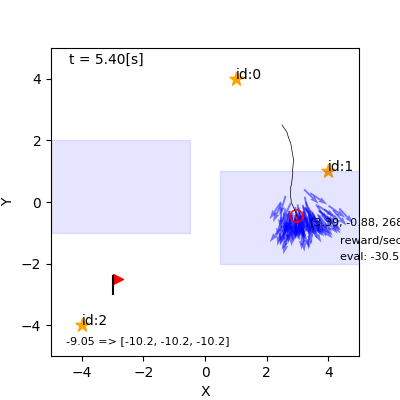
\includegraphics[width=1.0\linewidth]{figs/puddle_world.png}
  \vspace*{-4mm}
  \caption{Tensile stress-strain diagram}
  \label{fig: fig1}
\end{figure}


\footnotesize
\begin{thebibliography}{99}

\bibitem{Shinjuku98}
新宿大五朗,渋谷次郎,東京 学,``キャスティングマニピュレーションに関する研究(第1報,可変長の紐状柔軟リンクを有するマニピュレータの提案とそのスイング制御法)'',機論C編, vol.64-626, pp.3854--3861, 1998.

\bibitem{Shinjuku99}
Shinjuku, D., Shibuya, J. and Tokyo, M., ``Swing Motion Control of Casting Manipulation,'' IEEE Control Systems, vol.19-4, pp.56--64, 1999.

\end{thebibliography}

\normalsize
\end{document}
